\chapter{Application}
\label{chapter:application}
In this chapter we are going to have an in-depth look at the architecture of our application - \textbf{ExtWatcher}, that represents a solution for the enunciated problem in this thesis.


\section{Design}
\label{section:design}
\textit{ExtWatcher} is a software application assembled from multiple components with different used technologies (see Figure \ref{deployment}). In the following we will introduce you into it's implementation design starting from the low level and we will explain what role each component plays in the context of providing a truly effective security solution. 

\begin{figure}[H]
	\centerline{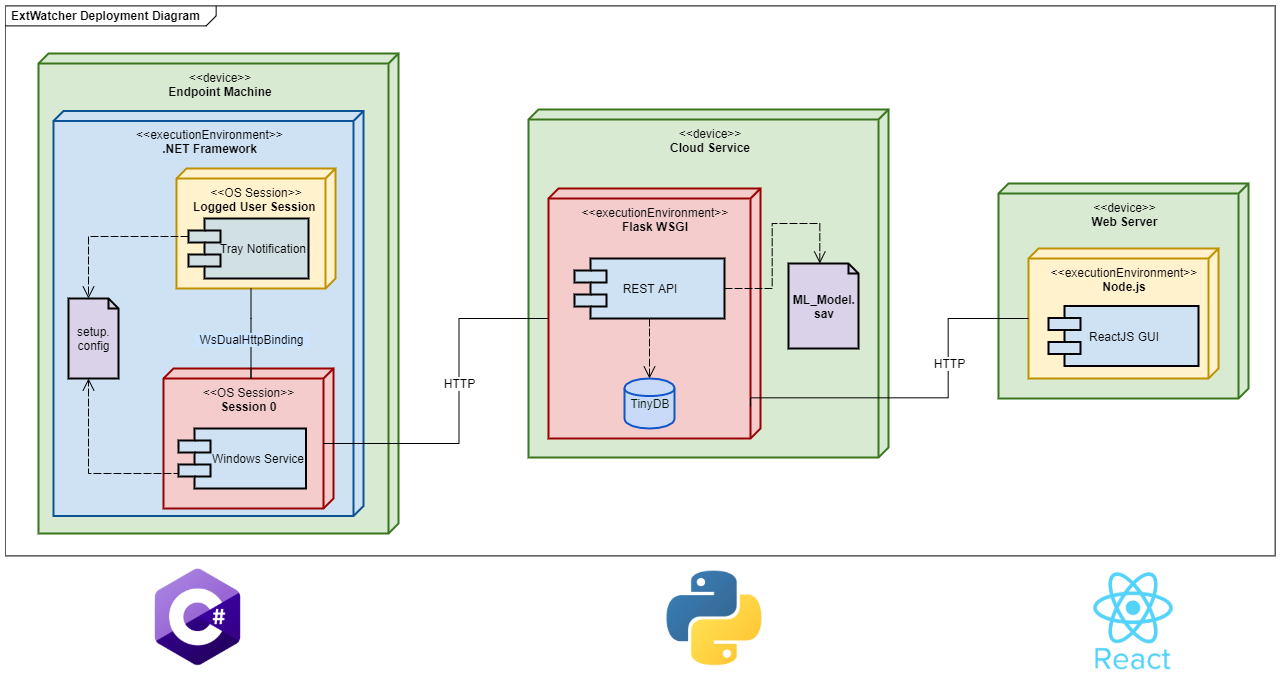
\includegraphics[scale=0.4]{figures/deployTech.png}}  
	\caption{Deployment Diagram of the application and used technologies}
	\label{deployment}
\end{figure}




\section{Windows Service}
\label{section:winService}

% Before putting to disposition of the user this tool, we had to create an installer (++ winService)

\begin{figure}[H]
	\centerline{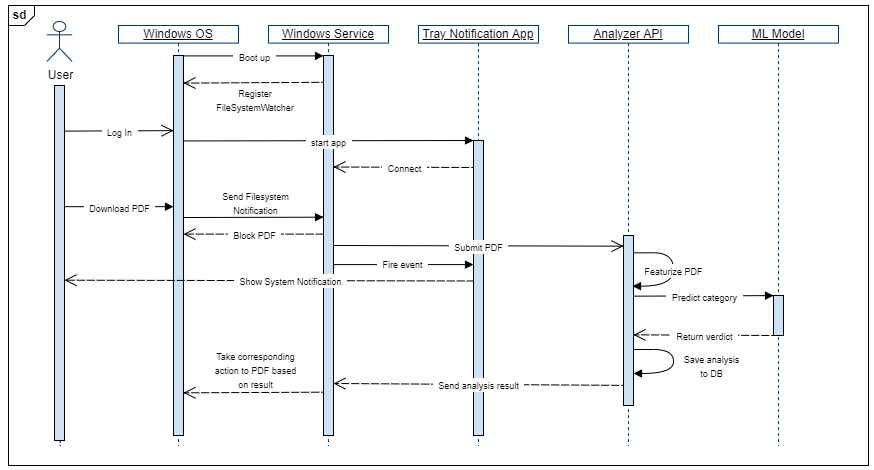
\includegraphics[scale=0.55]{figures/sequence.png}}  
	\caption{Sequence Diagram showing interaction between User, Windows Service and Cloud Analyzer}
	\label{sequence}
\end{figure}


\section{Cloud Analyzer}
\label{section:cloudApi}


\section{Dashboard Interface}
\label{section:dashboard}

\begin{figure}[H]
	\centerline{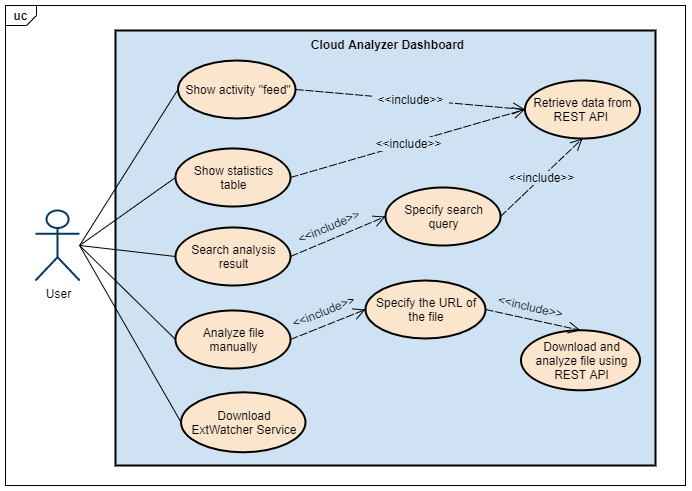
\includegraphics[scale=0.7]{figures/usecaseGUI.png}}  
	\caption{Use Case Diagram showing interaction between User and Cloud Analyzer using web GUI}
	\label{usecase}
\end{figure}